% Chapter Template

\chapter{Approach and Tools} % Main chapter title

\label{Chapter2} % Change X to a consecutive number; for referencing this chapter elsewhere, use \ref{ChapterX}

\lhead{Chapter 2. \emph{Approach and Tools}} % Change X to a consecutive number; this is for the header on each page - perhaps a shortened title

%----------------------------------------------------------------------------------------
%	SECTION 1
%----------------------------------------------------------------------------------------

\section{Approach}


%-----------------------------------
%	SUBSECTION 1
%-----------------------------------
\subsection{Network Model}
\label{sec:model}
Naturally occurring topologies like protein chains, cooperation networks and social networks follow scale-free structures, hence it was an obvious choice for modelling the network. For this purpose, the B-A model was followed, which also proposes variants of the scale free structure depending on its characteristics. These characteristics are : 

\begin{enumerate}
\item Continuous Growth (CG)
This characteristic marks that the network grows continuously. i.e., at all times, new nodes are being attached to the network. At the beginning of the simulation, the network only has a small number of nodes and this is known as the \textit{seed network}, and with time, new nodes are introduced in the network and it grows in size. The author uses a \textit{fully-connected network} as a seed network. Fully-connected network means each node of the network is connected to every other node in the network. It is to be noted here that the size of the network remains static throughout the simulation.

\item Preferential Attachment (PA)
This characteristic formulates the rule an incoming node should follow while making new connections within the network. It states that the most connected nodes are the most likely candidates for forming a new connection with. This leads on to a \textit{`rich gets richer'} tendency, and highly connected hubs are formed.
The connections are formed according to a probability value which is calculated as :

\begin{eqnarray}
 p_i = \frac{k_i}{\sum_{j=1}^{N} k_j} 
\label{eqn:PA}
\end{eqnarray}


where, 

\begin{enumerate}
\item p : probability 
\item k : number of connections 
\item i : agent id 
\item N : total number of agents 
\end{enumerate}

\end{enumerate} 

A scale free network may exhibit either or both of the above characteristics. However, the author decided to include both attributes in his model to make it as close to real life situations as possible.

%-----------------------------------
%	SUBSECTION 2
%-----------------------------------
\subsection{Orientation and View of the simulation environment}

Initially, an object-oriented view was used in the model to give better control over the agents in the network. But this led to very high time complexity, and the author chose to switch to a connection-oriented view of the model, where more focus was given to the connections being formed and everything was managed according to that view. This resulted in significant decrease in time complexity.
Also, focusing on the connections was easier as the whole network could be minimally represented by using the edge list.

Throughout the simulation, the network is represented by an edge list. It is a list, where each entry is a vector, and minimally this vector is a pair of two identification numbers referring to two distinct nodes. The presence of such a pair indicates the presence of a connection between the two nodes. It is notable that the values are always distinct, and this eliminates any chance of self-looping within the network. Optionally, the entries may contain other properties of the particular connection that may be used at different stages throughout the simulation.

These connections are treated as a probabilistic possibility for a communication between the nodes. However, presence of such a connection does not ensure that a communication takes place. The actual communication depends on more factors and more conditions need to be satisfied for that. These conditions are explained in detail in the next chapter~\ref{Chapter3}.

%-----------------------------------
%	SUBSECTION 3
%-----------------------------------

%\subsection{The Model}
%The author surmised to focus on a competitive diffusion where the companies compete over a single attribute of the agent. The attribute \emph{color} was chosen for the simulation as it is easy to understand and visualise, and it enabled the author to present the effect in a 2-dimensional spatial model where clustering is not directly dependent on the axial values. 
%As a limiting case, the author simulated only two companies. This limits the scope as it does not give much insight into cases where two companies might collaborate for mutual benefit, like to win against a third rival company.
%
%The model makes use of random functions wherever possible and applicable, and uses this to simulate the effect of `chance'. This inherent randomness makes the system non-deterministic and more reliable for the purpose of simulating more naturalistic occurrences.


%-----------------------------------
%	SUBSECTION 4
%-----------------------------------

\subsection{Presentation Approach}
\label{sec:presentaion}

\begin{figure}
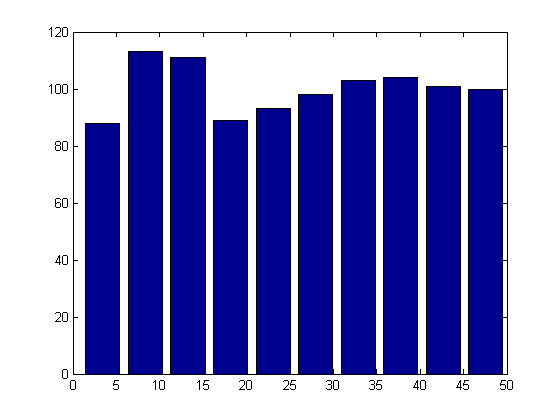
\includegraphics[scale=1]{Figures/1000_agents_color_cluster}
\caption{Colour Clusters}
\label{fig:color_clusters}
\end{figure}


Due to the large number of agents, a clear and easy way to understand presentation of the simulation was imperative.
Initially, the author went with 2-D histograms depicting the membership values of each color group, which accurately presented how the members move around as the height of the bars representing the number of members in a group could be easily seen to rise or fall, and the speed of this descent or ascent would tell about the rate of success or failure for a particular color. An example could be seen in figure~\ref{fig:color_clusters}.

\begin{figure}
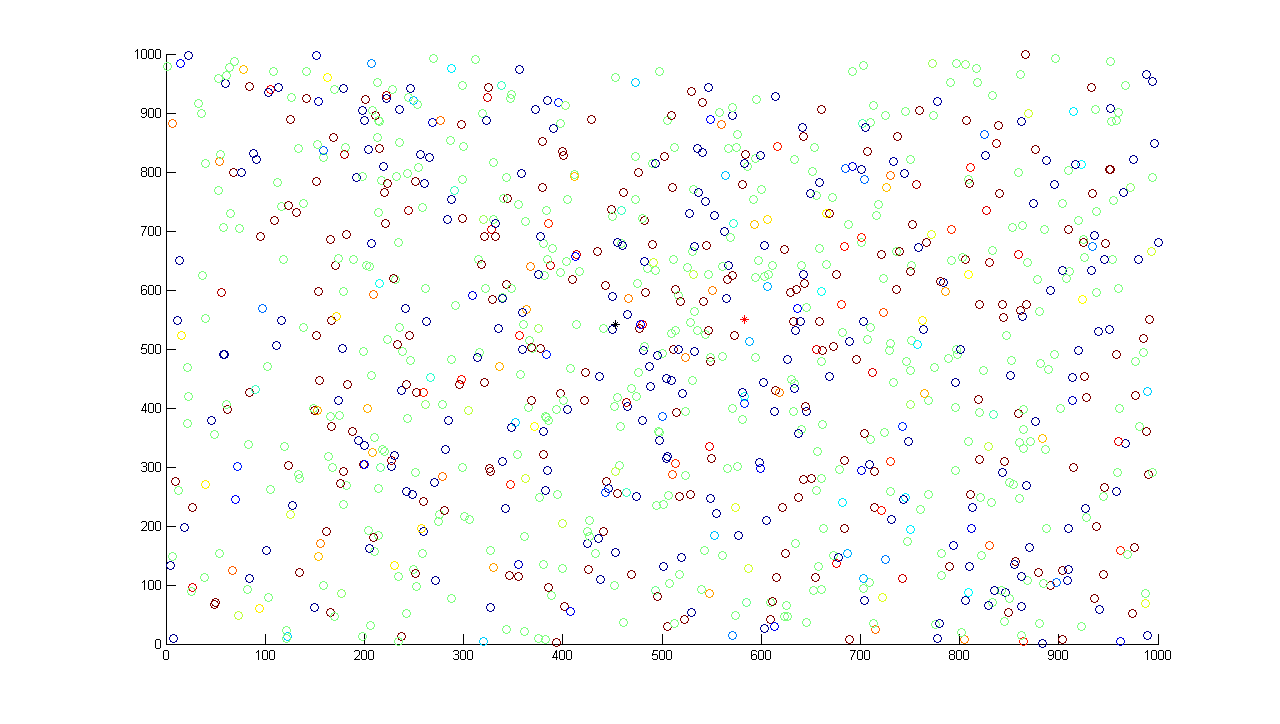
\includegraphics[scale=0.5]{Figures/spatial}
\caption{3-D Spatial Cluster}
\label{fig:spatial_clusters}
\end{figure}



However, with the progress of the model this representation became obsolete as it was unable to represent the aspect of ``Cost" to a company. 
To address this necessity, the author decided to switch to a 3-Dimensional presentation, with X- and Y- axes representing generic movement for agents, and the movement or effort as well as incurred cost for the companies. The color, being the third dimension of the presentation, depicts the value of the attribute and shows how an agent is leaning towards a company. The speed of movement here serves the purpose as the speed of rise/fall in the previous model. An example of this is figure ~\ref{fig:spatial_clusters}.

While the X-Y movement in this model is a correlation for the agents, the changing colors as they move represent the agents leaning towards or away from a particular company.

%-----------------------------------
%	SUBSECTION 5
%-----------------------------------
\subsection{Company Policies}
\label{sec:policies}
Different companies may have different policies towards customer involvement. These decisions are internal matters for them. However, Ives \& Olson ~\cite{1984} broadly divide the different approaches in six categories.
These categories are :

\begin{enumerate}

\item[1] No involvement. Users are unwilling or not invited to participate.
\item[2] Symbolic involvement. User input is requested but ignored. 
\item[3] Involvement by advice. User advice is solicited through interviews
or questionnaires.
\item[4]  Involvement by weak control. Users have sign-off responsibility at
each stage of the system development process. 
\item[5] Involvement by doing. A user as design team member or as the
official liaison with the information system's development group. 
\item[6] Involvement by strong control. Users may pay directly for new
development output from their own budget or the user's overall
organizational performance evaluation is dependent on the
outcome of the development effort. 
\end{enumerate}

The customer involvement continuum followed by the author follows the above categorisation and is influenced by the work of Bodil Sanden~\cite{bodil}, which argues that \textit{interaction is essential to customer involvement, specially in development of new sevices}.

Out of these, this thesis focuses on categories 2 and 5.
These two specific categories were chosen because they represent most dissimilar choices while still avoiding the extreme conditions, which allows the model to simulate the more probable scenarios.

%-----------------------------------
%	SUBSECTION 6
%-----------------------------------
\subsection{Simulation Approach}
The author surmised to focus on a competitive diffusion where the companies compete over a single attribute of the agent. The attribute \emph{color} was chosen for the simulation as it is easy to understand and visualise, and it enabled the author to present the effect in a 2-dimensional spatial model where clustering is not directly dependent on the axial values. 
As a limiting case, the author simulated only two companies. This limits the scope as it does not give much insight into cases where two companies might collaborate for mutual benefit, like to win against a third rival company. This model makes use of random functions wherever possible and applicable, and uses this to simulate the effect of `chance'. This inherent randomness makes the system non-deterministic and more reliable for the purpose of simulating more naturalistic occurrences.

The simulation focuses on companies attracting agents towards their cause, and the cost incurred in terms of efforts on the part of the company.
The model witnesses three types of potential interactions : 
\begin{enumerate}
\item[1] Company to Agent interaction 

These interactions are predefined, in a sense that a certain number of agents are already seeded to believe in a company at the beginning of the simulation. This is explained further in Chapter ~\ref{Chapter3}. This helps in creating an established base of users for the company. During the initial seeding, both companies are seeded with equal number of agents randomly chosen from the whole system and it is taken care of that there is no overlap in this initial customer base, i.e., all the agents being seeded are unique.

\item[2] Agent to Agent interactions

These interactions are the means by which one agent \textit{may influence} another to lean towards a company. In this model, the agents belonging to either of the companies in question are referred to as  \emph{influencing agents}, and the others are referred to as \emph{influenced agents}. This also mimics real life as the connections between agents are directional. The \textit{influencing agent} tries to motivate the \textit{influenced agent} to move towards its parent company, but the success or failure is decided based on a certain threshold value. This value depicts traits of the \textit{influencing agent} in question and the threshold is decided randomly, depicting traits of the \textit{influenced agent} and external factors such as luck and chance.

\item[3] Agent to Company interactions

Whenever an \textit{influenced agent} is successfully influenced during the simulation, this also causes the company to make some effort, the amount of which depends on its policies. These interactions are what cause the cost to the company. 

It is to be noted here that the \textit{influenced agent} in question need not be a new addition to the customer base of the company. It may already be a customer, however, further successful influence means that its loyalty towards the company is increased, which is denoted by a decrease in the distance between the agent and the company. 


\end{enumerate}

The outcome of these interactions are measured by the following two values:

\begin{enumerate}
\item[a] Gain

This refers to a company successfully influencing an agent to lean towards itself. 
For the purpose of this thesis, an incremental counter is used for every successful influence by an \textit{influencing agent}. 

For better results, a weighted function using the cumulative distance of the agents from the companies could be  used. However, the same is beyond the scope of this thesis.

\item[b] Cost

This refers to the cost incurred to the company and is a function of the effort made by the company. It depends on the policy being followed by the company.

In this thesis, the cost is represented by the work being done by the company in every step and is an abstract concept, without the notion of any budget. For a deeper analysis, a function of the total displacement of the company in every time step with relation to the initial position may be used. 
\end{enumerate}
	





%-----------------------------------
%	SECTION 2
%-----------------------------------

\section{Tools}
As a requirement from the University, Matlab was chosen as the programming language, and no special toolboxes were used.
The curve fitting application was used occasionally to check the output of the simulation.

The formulas, and variants thereof, used by the author were sometimes first tested as a prototype in Python with NetworkX and Mathematica for mathematical validation. However, any of those implementations do not directly contribute to the result.
